\documentclass{amsart}
\usepackage{amsmath, amssymb, amsthm}
\usepackage{tikz}
\usepackage{geometry}
\geometry{margin=1in}

\newtheorem*{claim}{Claim}

\title{Homework 1}
\author{Richard Harnisch \\ s5238366}

\begin{document}
\maketitle

\textbf{Problem.} Assume that the functions $c : \mathbb{R} \to \mathbb{R}$ and $f : \mathbb{R} \to \mathbb{R}$ are continuous. Consider the following initial value problem:
\[
  \frac{\partial u}{\partial t} + c(x)\frac{\partial u}{\partial x} = 0, \quad u(0, x) = f(x).
\]
Assume that the characteristic curve through the point $(0, 0)$ in the $(t, x)$-plane is a strictly increasing function of $t$ and has the lines $x = h_1$ and $x = h_2$, where $h_1 < 0 < h_2$, as horizontal asymptotes.

\begin{enumerate}
  \item[(a)] Fix $a \in (h_1, h_2)$. Draw a qualitatively correct sketch in the $(t, x)$-plane showing the characteristic curves that pass through the points $(t_1, a)$ and $(t_2, a)$, where $0 < t_1 < t_2$, together with their asymptotes.

  \item[(b)] Let $(t_n)$ be any strictly increasing sequence such that $t_n \to \infty$. Show that $\lim_{n \to \infty} u(t_n, a)$ exists.
\end{enumerate}

\bigskip
\textbf{Solution.}

\textbf{Setup via characteristics.}
The PDE $u_t + c(x)u_x = 0$ is solved by the method of characteristics. Along a curve $(t, x(t))$ satisfying
\[
  \frac{dx}{dt} = c(x),
\]
the total derivative of $u$ is zero, so $u$ is constant. Let $\varphi : \mathbb{R} \to (h_1, h_2)$ denote the characteristic through $(0,0)$:
\[
  \frac{d\varphi}{dt} = c(\varphi(t)), \quad \varphi(0) = 0.
\]
By hypothesis, $\varphi$ is strictly increasing, $\varphi(t) \to h_2$ as $t \to +\infty$, and $\varphi(t) \to h_1$ as $t \to -\infty$. In particular, $c(h_1) = c(h_2) = 0$ and $c(x) > 0$ for $x \in (h_1, h_2)$.

Because the ODE is autonomous, the characteristic through any point $(0, x_0)$ with $x_0 \in (h_1, h_2)$ is $t \mapsto \varphi(t + s_0)$, where $s_0$ is the unique value satisfying $\varphi(s_0) = x_0$. Thus every characteristic is a time-translate of $\varphi$ and shares the same asymptotes $x = h_1$ and $x = h_2$.

\medskip
\textbf{Part (a).}

Fix $a \in (h_1, h_2)$ and let $\tau_a \in \mathbb{R}$ be the unique value with $\varphi(\tau_a) = a$. The characteristic through $(t_i, a)$ is $t \mapsto \varphi(t - t_i + \tau_a)$, a rightward shift of $\varphi$ by $t_i - \tau_a$. Since $0 < t_1 < t_2$, the curve through $(t_2, a)$ is shifted further to the right than the one through $(t_1, a)$.

\begin{center}
  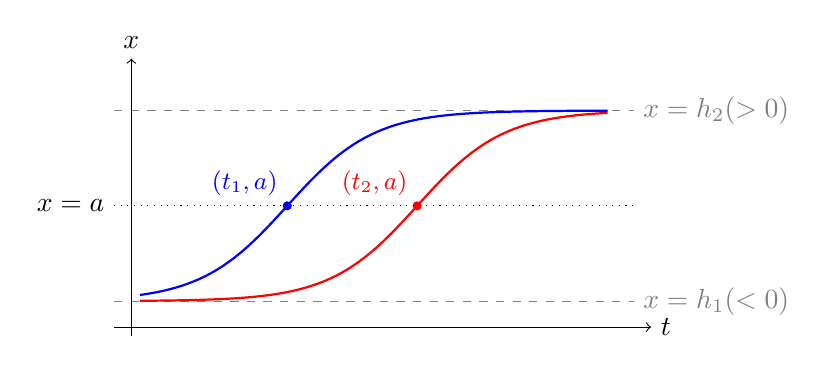
\begin{tikzpicture}[scale=1.1]
    % Asymptotes
    \draw[dashed, gray] (-0.5, 2.2) -- (5.5, 2.2) node[right] {$x = h_2 (> 0)$};
    \draw[dashed, gray] (-0.5, 0.0) -- (5.5, 0.0) node[right] {$x = h_1 (< 0)$};

    % Characteristic through (t1, a): centered so it passes through (1.5, 1.1)
    % Use a shifted sigmoid-like curve: x(t) = h1 + (h2-h1)/(1 + exp(-k(t - shift)))
    % h1=0, h2=2.2, through (t1,a) = (1.5, 1.1)
    % 1.1 = 2.2/(1+exp(-k*0)) => exp(0)=1 => 1.1=1.1 check, shift=1.5
    \draw[blue, thick, domain=-0.2:5.2, samples=80]
    plot (\x, {2.2 / (1 + exp(-2*(\x - 1.5)))})
    node[right] {};
    \fill[blue] (1.5, 1.1) circle (1.5pt) node[above left] {\small$(t_1,a)$};

    % Characteristic through (t2, a): shift = 3.0
    \draw[red, thick, domain=-0.2:5.2, samples=80]
    plot (\x, {2.2 / (1 + exp(-2*(\x - 3.0)))})
    node[right] {};
    \fill[red] (3.0, 1.1) circle (1.5pt) node[above left] {\small$(t_2,a)$};

    % Dashed horizontal at a
    \draw[dotted] (-0.5, 1.1) node[left] {$x = a$} -- (5.5, 1.1);

    % Axes
    \draw[->] (-0.3, -0.4) -- (-0.3, 2.8) node[above] {$x$};
    \draw[->] (-0.5, -0.3) -- (5.7, -0.3) node[right] {$t$};
  \end{tikzpicture}
\end{center}

Both curves are strictly increasing, approach $x = h_1$ as $t \to -\infty$, and approach $x = h_2$ as $t \to +\infty$. The curve through $(t_2, a)$ is the rightward translate of the one through $(t_1, a)$.

\medskip
\textbf{Part (b).}

\begin{claim}
  For any strictly increasing sequence $(t_n)$ with $t_n \to \infty$, we have $\displaystyle\lim_{n\to\infty} u(t_n, a) = f(h_1)$.
\end{claim}

\begin{proof}
  Fix $a \in (h_1, h_2)$, and let $\tau_a$ be the unique real number satisfying $\varphi(\tau_a) = a$.

  For each $n$, let $x_n \in (h_1, h_2)$ denote the initial position of the characteristic that passes through $(t_n, a)$; that is, $x_n$ satisfies $\varphi(t_n + s_n) = a$ where $\varphi(s_n) = x_n$. Since $\varphi$ is a bijection from $\mathbb{R}$ to $(h_1, h_2)$, we obtain
  \[
    t_n + s_n = \tau_a \implies s_n = \tau_a - t_n,
  \]
  so
  \[
    x_n = \varphi(\tau_a - t_n).
  \]

  Because $u$ is constant along characteristics, $u(t_n, a) = u(0, x_n) = f(x_n)$. Therefore
  \[
    \lim_{n \to \infty} u(t_n, a) = \lim_{n \to \infty} f\!\left(\varphi(\tau_a - t_n)\right).
  \]

  Since $t_n \to \infty$, we have $\tau_a - t_n \to -\infty$. By hypothesis, $\varphi(t) \to h_1$ as $t \to -\infty$, so $\varphi(\tau_a - t_n) \to h_1$. By continuity of $f$,
  \[
    \lim_{n \to \infty} f\!\left(\varphi(\tau_a - t_n)\right) = f(h_1).
  \]

  Hence $\lim_{n\to\infty} u(t_n, a) = f(h_1)$, which in particular shows the limit exists and is independent of the choice of sequence $(t_n)$.
\end{proof}

\end{document}
